% !TEX program = pdflatex
% !TEX options = -synctex=1 -interaction=nonstopmode -file-line-error "%DOC%"
% 固体物理第六次作业
\documentclass[UTF8,10pt,a4paper]{article}
\usepackage{ctex}
% \catcode`\。=\active
% \newcommand{。}{.}
\newcommand{\CourseName}{固体物理}
\newcommand{\CourseCode}{PHYS1502}
\newcommand{\Semester}{2019-2020学年第二学期}
\newcommand{\ProjectName}{第六次作业}
\newcommand{\DueTimeType}{截止时间}
\newcommand{\DueTime}{2020. 4. 17(周五)17:00}
\newcommand{\StudentName}{陈稼霖}
\newcommand{\StudentID}{45875852}
\usepackage[vmargin=1in,hmargin=.5in]{geometry}
\usepackage{fancyhdr}
\usepackage{lastpage}
\usepackage{calc}
\pagestyle{fancy}
\fancyhf{}
\fancyhead[L]{\CourseName}
\fancyhead[C]{\ProjectName}
\fancyhead[R]{\StudentName}
\fancyfoot[R]{\thepage\ / \pageref{LastPage}}
\setlength\headheight{12pt}
\fancypagestyle{FirstPageStyle}{
    \fancyhf{}
    \fancyhead[L]{\CourseName\\
        \CourseCode\\
        \Semester}
    \fancyhead[C]{{\Huge\bfseries\ProjectName}\\
        \DueTimeType\ : \DueTime}
    \fancyhead[R]{姓名 : \makebox[\widthof{\StudentID}][s]{\StudentName}\\
        学号 : \StudentID\\
        成绩 : \underline{\makebox[\widthof{\StudentID}]{}}}
    \fancyfoot[R]{\thepage\ / \pageref{LastPage}}
    \setlength\headheight{36pt}
}
\usepackage{amsmath,amssymb,amsthm,bm}
\allowdisplaybreaks[4]
\newtheoremstyle{Problem}
{}
{}
{}
{}
{\bfseries}
{.}
{ }
{第\thmnumber{ #2}\thmname{ #1}\thmnote{ (#3)} 得分: \underline{\qquad\qquad}}
\theoremstyle{Problem}
\newtheorem{prob}{题}
\newtheoremstyle{Solution}
{}
{}
{}
{}
{\bfseries}
{:}
{ }
{\thmname{#1}}
\makeatletter
\def\@endtheorem{\qed\endtrivlist\@endpefalse}
\makeatother
\theoremstyle{Solution}
\newtheorem*{sol}{解}
\providecommand{\abs}[1]{\left\lvert#1\right\rvert}
\usepackage{graphicx}
\usepackage{subfigure}
\begin{document}
\thispagestyle{FirstPageStyle}
\begin{prob}[(10.1) Normal modes of a One-Dimensional Diatomic Chain]
    \begin{enumerate}
        \item[(a)] What is the difference between an acoustic mode and an optical mode.
        \begin{itemize}
            \item[$\triangleright$] Describe how particles move in each case.
        \end{itemize}
    \end{enumerate}
    \item[(b)] Derive the dispersion relation for the longitudinal oscillations of a one-dimensional diatomic mass-and-spring crystal where the unit cell is of length $a$ and each unit cell contains one atom of mass $m_1$ and one atom of mass $m_2$ connected together by springs with spring constant $\kappa$, as shown in the figure (all springs are the same, and motion of particles is in one dimensions only).
    \begin{figure}[h]
        \centering
        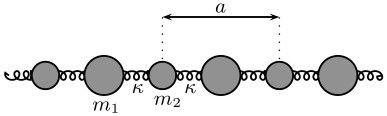
\includegraphics[width=.4\textwidth]{1.png}
    \end{figure}
    \item[(c)] Determine the frequencies of the acoustic and optical modes at $k=0$ as well as the Brillouin zone boundary.
    \begin{itemize}
        \item[$\triangleright$] Describe the motion of the masses in each case (see margin note 4 of this chapter!).
        \item[$\triangleright$] Determine the sound velocity and show that the group velocity is zero at the zone boundary.
        \item[$\triangleright$] Show that the sound velocity is also given by $v_s=\sqrt{\beta^{-1}/\rho}$ where $\rho$ is the chain density and $\beta$ is the compressibility.
    \end{itemize}
    \item[(d)] Sketch the dispersion in both reduced and extended zone scheme.
    \begin{itemize}
        \item[$\triangleright$] If there are $N$ unit cells, how many different normal modes are there?
        \item[$\triangleright$] How many \textit{branches} of excitations are there? I.e., in reduced zone scheme, how many modes are there at each $k$?
    \end{itemize}
    \item[(e)] What happens when $m_1=m_2$?
\end{prob}
\begin{sol}
    \begin{enumerate}
        \item[(a)] 声学模是色散关系中能量较高的一支,而光学模是色散关系中能量较低的一支. 声学模描述原胞质心的振动,而光学模描述原胞内原子的相对振动.
        \begin{itemize}
            \item[$\triangleright$] 对于一维双原子链,声学模中原胞内的原子以缓慢的空间调制同相运动,长波极限下,所有原子同向运动. 光学模中原胞内的原子以缓慢的空间调制异向运动,长波极限下同一个原胞中的原子反向运动.
        \end{itemize}
        \item[(b)] 设第$n$个原胞中两个原子的坐标分别为$x_n$和$y_n$,其偏离平衡位置的位移分别为$\delta x_x$和$\delta y_n$,运动方程分别为
        \begin{align}
            m_1\ddot{x_n}=&\kappa(\delta y_{n-1}-\delta x_n)+\kappa(\delta y_n-\delta x_n),\\
            m_2\ddot{y_n}=&\kappa(\delta x_n-\delta y_n)+\kappa(\delta x_{n+1}-\delta y_n).
        \end{align}
        设
        \begin{align}
            \delta x_n=&A_xe^{i(\omega t-kna)},\\
            \delta y_n=&A_ye^{i(\omega t-kna)}.
        \end{align}
        将上面两式代入运动方程中得
        \begin{align}
            -m_1\omega^2A_x=\kappa(A_ye^{ika}-A_x)+\kappa(A_y-A_x),\\
            -m_2\omega^2A_y=\kappa(A_x-A_y)+\kappa(A_xe^{ika}-A_y).
        \end{align}
        将上面两式转化为线性代数形式得
        \begin{align}
            \omega^2\left(\begin{matrix}
                A_x\\
                A_y
            \end{matrix}\right)=\left(\begin{matrix}
                \frac{2\kappa}{m_1}&-\frac{\kappa}{m_1}(1+e^{i\kappa a})\\
                -\frac{\kappa}{m_2}(1+e^{-i\kappa a})&\frac{2\kappa}{m_2}
            \end{matrix}\right)\left(\begin{matrix}
                A_x\\
                A_y
            \end{matrix}\right).
        \end{align}
        下面求解上式右侧矩阵的本征值
        \begin{align}
            \nonumber\abs{\begin{matrix}
                \frac{2\kappa}{m_1}-\omega^2&-\frac{\kappa}{m_1}(1+e^{ika})\\
                -\frac{\kappa}{m_2}(1+e^{-ika})&\frac{2\kappa}{m_2}-\omega^2
            \end{matrix}}=&\omega^4-2\kappa\left(\frac{1}{m_1}+\frac{1}{m_2}\right)+\frac{\kappa^2}{m_1m_2}\left(2-2\cos ka\right)\\
            =&\omega^4-2\kappa\left(\frac{1}{m_1}+\frac{1}{m_2}\right)+\frac{4\kappa^2}{m_1m_2}\sin^2\left(\frac{ka}{2}\right)=0,
        \end{align}
        解得
        \begin{align}
            \nonumber\omega_{\pm}^2=&\kappa\left[\left(\frac{1}{m_1}+\frac{1}{m_2}\right)\pm\sqrt{\left(\frac{1}{m_1}+\frac{1}{m_2}\right)^2-\frac{4}{m_1m_2}\sin^2\left(\frac{ka}{2}\right)}\right]\\
            =&\frac{\kappa}{m_1m_2}\left[(m_1+m_2)\pm\sqrt{(m_1+m_2)^2-4m_1m_2\sin^2\left(\frac{ka}{2}\right)}\right].
        \end{align}
        故一维双原晶体纵波的色散关系为
        \begin{align}
            \omega_{\pm}=&\sqrt{\frac{\kappa}{m_1m_2}\left[(m_1+m_2)\pm\sqrt{(m_1+m_2)^2-4m_1m_2\sin^2\left(\frac{ka}{2}\right)}\right]},
        \end{align}
        其中下标$-$代表声学模,$+$代表光学模.
        \item[(c)] 声学模在$k=0$处的频率为
        \begin{align}
            \omega_-(0)=0.
        \end{align}
        光学模在$k=0$处的频率为
        \begin{align}
            \omega_+(0)=\sqrt{\frac{2\kappa(m_1+m_2)}{m_1m_2}}.
        \end{align}
        在布里渊区边界处($k=\pm\frac{\pi}{a}$),声学模的频率为
        \begin{align}
            \omega_-(\pm\frac{\pi}{a})=\sqrt{\frac{2\kappa\min\{m_1,m_2\}}{m_1m_2}}.
        \end{align}
        光学模的频率为
        \begin{align}
            \omega_+(\pm\frac{\pi}{a})=\sqrt{\frac{2\kappa\max\{m_1,m_2\}}{m_1m_2}}.
        \end{align}
        \begin{itemize}
            \item[$\triangleright$] 当$k=0$时,对于声学模,上面的线性代数形式的运动方程化为
            \begin{align}
                0=2\kappa\left(\begin{matrix}
                    \frac{1}{m_1}&-\frac{1}{m_1}\\
                    -\frac{1}{m_2}&\frac{1}{m_2}
                \end{matrix}\right)\left(\begin{matrix}
                    A_x\\
                    A_y
                \end{matrix}\right),
            \end{align}
            故
            \begin{align}
                A_x=A_y.
            \end{align}
            同一个原胞中两个原子振幅相等,运动方向相同.\\
            对光学模,则有
            \begin{align}
                \frac{2\kappa(m_1+m_2)}{m_1m_2}=2\kappa\left(\begin{matrix}
                    \frac{1}{m_1}&\frac{1}{m_1}\\
                    \frac{1}{m_2}&\frac{1}{m_2}
                \end{matrix}\right)\left(\begin{matrix}
                    A_x\\
                    A_y
                \end{matrix}\right),
            \end{align}
            故
            \begin{align}
                \frac{A_x}{A_y}=-\frac{m_2}{m_1}.
            \end{align}
            同一个原胞内两个原子振幅之比为$\frac{m_2}{m_1}$(原子越重,振幅越小),方向相反.\\
            在布里渊区边界处,对于声学模,
            \begin{align}
                \frac{2\kappa\min\{m_1,m_2\}}{m_1m_2}\left(\begin{matrix}
                    A_x\\
                    A_y
                \end{matrix}\right)=\left(\begin{matrix}
                    \frac{2\kappa}{m_1}&0\\
                    0&\frac{2\kappa}{m_2}
                \end{matrix}\right)\left(\begin{matrix}
                    A_x\\
                    A_y
                \end{matrix}\right),
            \end{align}
            故
            \begin{align}
                A_x&\left\{\begin{array}{ll}
                    =0,&m_1\leq m_2,\\
                    =\text{任意值},&m_1>m_2.
                \end{array}\right.\\
                A_y&\left\{\begin{array}{ll}
                    =\text{任意值},&m_1\leq m_2,\\
                    =0,&m_1>m_2.
                \end{array}\right.
            \end{align}
            同一个原胞内质量大的那个原子振动,而另一个原子不动.\\
            对于光学模,
            \begin{align}
                \frac{2\kappa\max{m_1,m_2}}{m_1m_2}\left(\begin{matrix}
                    A_x\\
                    A_y
                \end{matrix}\right)=\left(\begin{matrix}
                    \frac{2\kappa}{m_1}&0\\
                    0&\frac{2\kappa}{m_2}
                \end{matrix}\right)\left(\begin{matrix}
                    A_x\\
                    A_y
                \end{matrix}\right),
            \end{align}
            故
            \begin{align}
                A_x&\left\{\begin{array}{ll}
                    =\text{任意值},&m_1\leq m_2,\\
                    =0,&m_1>m_2.
                \end{array}\right.\\
                A_y&\left\{\begin{array}{ll}
                    =0,&m_1\leq m_2,\\
                    =\text{任意值},&m_1>m_2.
                \end{array}\right.
            \end{align}
            同一个原胞内质量小的那个原子振动,而另一个原子不动.
            \item[$\triangleright$] 一般地,声速为
            \begin{align}
                v_{\text{sound}}=\frac{d\omega_-}{dk}.
            \end{align}
            因为声波波长长,即$k\rightarrow 0$,声学模的频率可近似为
            \begin{align}
                \nonumber\omega_-=&\sqrt{\frac{\kappa}{m_1m_2}\left[(m_1+m_2)-\sqrt{(m_1+m_2)^2-4m_1m_2\sin^2\left(\frac{ka}{2}\right)}\right]}\\
                \nonumber=&\sqrt{\frac{\kappa(m_1+m_2)}{m_1m_2}\left[1-\sqrt{1-\frac{4m_1m_2}{(m_1+m_2)^2}\sin^2\left(\frac{ka}{a}\right)}\right]}\\
                \nonumber\approx&\sqrt{\frac{\kappa(m_1+m_2)}{m_1m_2}\left[1-1+\frac{2m_1m_2}{(m_1+m_2)^2}\sin^2\left(\frac{ka}{a}\right)\right]}\\
                =&\sqrt{\frac{2\kappa}{m_1+m_2}}\abs{\sin\left(\frac{ka}{2}\right)}.
            \end{align}
            声速为
            \begin{align}
                v_{\text{sound}}(0)=\left.\frac{d\omega_-}{dk}\right\rvert_{k=0}=\lim_{k\rightarrow 0}\frac{d\left[\sqrt{\frac{2\kappa}{m_1+m_2}}\sin(ka/2)\right]}{dk}=a\sqrt{\frac{\kappa}{2(m_1+m_2)}}.
            \end{align}
            光学模的群速度为
            \begin{align}
                v_{+,g}(0)=\left.\frac{d\omega_+}{dk}\right\rvert_{k=0}=\lim_{k\rightarrow 0}\frac{d\left[\sqrt{\frac{\kappa}{m_1m_2}\left[(m_1+m_2)+\sqrt{(m_1+m_2)^2-4m_1m_2\sin^2\left(\frac{ka}{2}\right)}\right]}\right]}{dk}=0.
            \end{align}
            \item[$\triangleright$] 原子链的线密度为
            \begin{align}
                \rho=\frac{m_1+m_2}{\rho}.
            \end{align}
            压缩系数为
            \begin{align}
                \beta=-\frac{1}{L}\frac{\partial L}{\partial F}=-\frac{1}{Na}\left(\frac{\partial F}{\partial Na}\right)^{-1}=-\frac{1}{a}\left(\frac{\partial F}{\partial a}\right)^{-1}=\frac{2}{a\kappa}.
            \end{align}
            故声速可以由下式得到
            \begin{align}
                v_s=\sqrt{\beta^{-1}/\rho}=a\sqrt{\frac{\kappa}{2(m_1+m_2)}}.
            \end{align}
        \end{itemize}
        \item[(d)] 色散关系的两种不同画法如图\ref{1-omega-k}.
        \begin{figure}[h]
            \centering
            \subfigure[简约布里渊区.]{
            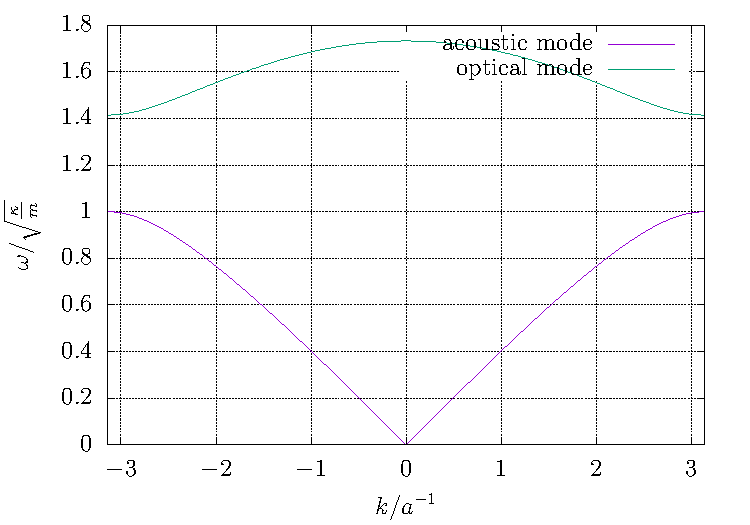
\includegraphics[width=.4\textwidth]{1-ReducedZoneScheme.pdf}}
            \subfigure[拓展布里渊区.]{
            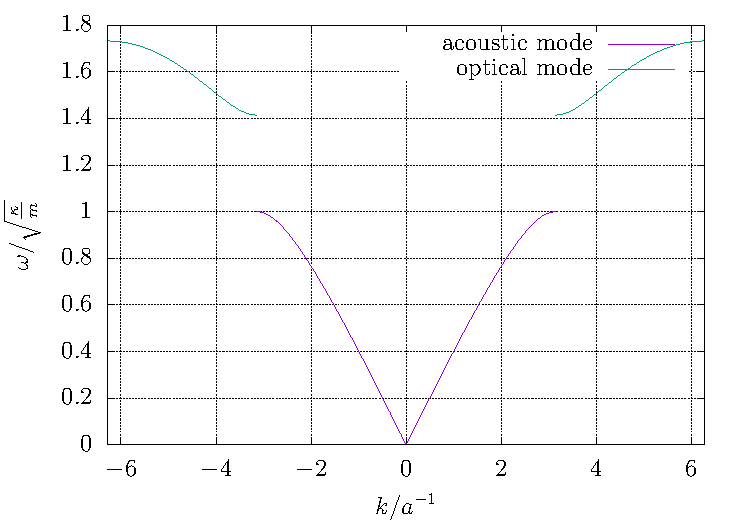
\includegraphics[width=.4\textwidth]{1-ExtendedZoneScheme.pdf}}
            \caption{色散关系的两种不同画法,其中设$m_1=2m$,$m_2=m$,横坐标$k$以$a^{-1}$为单位,纵坐标$\omega$以$\sqrt{\frac{\kappa}{m}}$为单位.}
            \label{1-omega-k}
        \end{figure}
        \begin{itemize}
            \item[$\triangleright$] 若有$N$个原胞,则有$2N$个不同的正则模式.
            \item[$\triangleright$] 在简约布里渊区内,对于给定的每个$k$,对应着$2$个模式,也就是说有$2$个分支的激发.
        \end{itemize}
        \item[(e)] 当$m_1=m_2$,系统由双原子链变为单原子链,每个原胞中仅含$1$个原子,在拓展布里渊区中,声学模和光学模的色散关系曲线连成一条,变为单原子链的色散关系曲线.
    \end{enumerate}
\end{sol}

\begin{prob}[(10.5) Triatomic Chain$^*$]
    Consider a mass-and-spring model with three different masses and three different springs per unit cell as shown in this diagram.
    \begin{figure}[h]
        \centering
        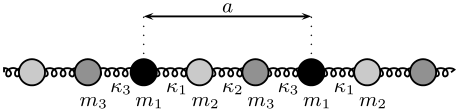
\includegraphics[width=.4\textwidth]{2.png}
    \end{figure}
    \begin{enumerate}
        \item[(a)] At $k=0$ how many optical modes are there? Calculate the energies of these modes. Hint: You will get a cubic equation. However, you already know one of the roots since it is the energy of the acoustic mode at $k=0$.
        \item[(b)$^*$] If all the masses are the same and $\kappa_1=\kappa_2$ determine the frequencies of all three modes at the zone boundary $k=\pi/a$. You will have a cubic equation, but you should be able to guess one root which corresponds to a particularly simple normal mode.
        \item[(c)$^*$] If all three spring constants are the same, and $m_1=m_2$ determine the frequencies of all three modes at the zone boundary $k=\pi/a$. Again you should be able to guess one of the roots.
    \end{enumerate}
\end{prob}
\begin{sol}
    \begin{enumerate}
        \item[(a)] 当$k=0$时,有$2$个光学模. 设第$n$个原胞中三个原子的坐标分别为$x_n$,$y_n$和$z_n$,其偏离平衡位置的位移分别为$\delta x_n$,$\delta y_n$和$\delta z_n$,运动方程分别为
        \begin{align}
            m_1\ddot{\delta x_n}=&\kappa_3(\delta z_{n-1}-\delta x_n)+\kappa_1(\delta y_n-\delta x_n),\\
            m_2\ddot{\delta y_n}=&\kappa_1(\delta x_n-\delta y_n)+\kappa_2(\delta z_n-\delta y_n),\\
            m_3\ddot{\delta z_n}=&\kappa_2(\delta y_n-\delta z_n)+\kappa_3(\delta x_{n+1}-\delta z_n).
        \end{align}
        设
        \begin{align}
            \delta x_n=&A_xe^{i(\omega t-kna)},\\
            \delta y_n=&A_ye^{i(\omega t-kna)},\\
            \delta z_n=&A_ze^{i(\omega t-kna)}.
        \end{align}
        将上面三式代入运动方程得
        \begin{align}
            -m_1\omega^2A_x=&\kappa_3(e^{ika}A_z-A_x)+\kappa_1(A_y-A_x),\\
            -m_2\omega^2A_y=&\kappa_1(A_x-A_y)+\kappa_2(A_z-A_y),\\
            -m_3\omega^2A_z=&\kappa_2(A_y-A_z)+\kappa_3(e^{-ika}A_x-A_z).
        \end{align}
        将上面三式化为线性代数形式得
        \begin{align}
            \omega^2\left(\begin{matrix}
                A_x\\
                A_y\\
                A_z
            \end{matrix}\right)=\left(\begin{matrix}
                \frac{\kappa_1+\kappa_2}{m_1}&-\frac{\kappa_1}{m_1}&-\frac{\kappa e^{ika}}{m_1}\\
                -\frac{\kappa_1}{m_2}&\frac{(\kappa_1+\kappa_2)}{m_2}&-\frac{\kappa_2}{m_2}\\
                -\frac{\kappa_3e^{ika}}{m_3}&-\frac{\kappa_2}{m_3}&\frac{\kappa_2+\kappa_3}{m_3}
            \end{matrix}\right)\left(\begin{matrix}
                A_x\\
                A_y\\
                A_z
            \end{matrix}\right).
        \end{align}
        下面求解上式右侧矩阵的本征值
        \begin{align}
            \label{2-CE}
            \nonumber&\abs{\begin{matrix}
                \frac{\kappa_3+\kappa_1}{m_1}-\omega^2&-\frac{\kappa_1}{m_1}&-\frac{\kappa_3}{m_1}e^{-ika}\\
                -\frac{\kappa_1}{m_2}&\frac{\kappa_1+\kappa_2}{m_2}-\omega^2&-\frac{\kappa_2}{m_2}\\
                -\frac{\kappa_3}{m_3}e^{ika}&-\frac{\kappa_2}{m_3}&\frac{\kappa_2+\kappa_3}{m_3}-\omega^2
            \end{matrix}}\\
            \nonumber=&-\omega^6+\left(\frac{\kappa_3+\kappa_1}{m_1}+\frac{\kappa_1+\kappa_2}{m_2}+\frac{\kappa_2+\kappa_3}{m_3}\right)\omega^4-\frac{(\kappa_1\kappa_2+\kappa_2\kappa_3+\kappa_3\kappa_1)(m_1+m_2+m_3)}{m_1m_2m_3}\omega^2\\
            &+\frac{\kappa_1\kappa_2\kappa_3}{m_1m_2m_3}(2-2\cos ka)=0.
        \end{align}
        当$k=0$时,
        \begin{align}
            -\omega^6+\left(\frac{\kappa_3+\kappa_1}{m_1}+\frac{\kappa_1+\kappa_2}{m_2}+\frac{\kappa_2+\kappa_3}{m_3}\right)\omega^4-\frac{(\kappa_1\kappa_2+\kappa_2\kappa_3+\kappa_3\kappa_1)(m_1+m_2+m_3)}{m_1m_2m_3}\omega^2=0,
        \end{align}
        且我们已知此时对声学模,$\omega_{\text{acoustic}}=0$,故另外两个光学模的频率由下式给出
        \begin{align}
            -\omega^4+\left(\frac{\kappa_3+\kappa_1}{m_1}+\frac{\kappa_1+\kappa_2}{m_2}+\frac{\kappa_2+\kappa_3}{m_3}\right)\omega^2-\frac{(\kappa_1\kappa_2+\kappa_2\kappa_3+\kappa_3\kappa_1)(m_1+m_2+m_3)}{m_1m_2m_3}=0,
        \end{align}
        解得
        \scriptsize
        \begin{align}
            \omega_{\text{optical},1/2}^2=\frac{1}{2}\left[\left(\frac{\kappa_1+\kappa_2}{m_1}+\frac{\kappa_1+\kappa_2}{m_2}+\frac{\kappa_2+\kappa_3}{m_3}\right)\pm\sqrt{\left(\frac{\kappa_1+\kappa_2}{m_1}+\frac{\kappa_1+\kappa_2}{m_2}+\frac{\kappa_2+\kappa_3}{m_3}\right)^2-\frac{4(\kappa_1\kappa_2+\kappa_2\kappa_3+\kappa_3\kappa_1)(m_1+m_2+m_3)}{m_1m_2m_3}}\right].
        \end{align}
        \normalsize
        故两个光学模的频率分别为
        \scriptsize
        \begin{align}
            \omega_{\text{optical},1/2}=\sqrt{\frac{1}{2}\left[\left(\frac{\kappa_1+\kappa_2}{m_1}+\frac{\kappa_1+\kappa_2}{m_2}+\frac{\kappa_2+\kappa_3}{m_3}\right)\pm\sqrt{\left(\frac{\kappa_1+\kappa_2}{m_1}+\frac{\kappa_1+\kappa_2}{m_2}+\frac{\kappa_2+\kappa_3}{m_3}\right)^2-\frac{4(\kappa_1\kappa_2+\kappa_2\kappa_3+\kappa_3\kappa_1)(m_1+m_2+m_3)}{m_1m_2m_3}}\right]}.
        \end{align}
        \normalsize
        \item[(b)] 当$m_1=m_2=m_3$且$\kappa_1=\kappa_2$时,在布里渊区边界处($k=\pm\frac{\pi}{a}$),式\eqref{2-CE}可化为
        \begin{align}
            \label{2-CE-2}
            -\omega^6+\frac{4\kappa_1+2\kappa_3}{m_1}\omega^4-\frac{3(\kappa_1^2+2\kappa_1\kappa_3)}{m_1^2}\omega^2+4\frac{\kappa_1^2\kappa_3}{m_1^3}=0.
        \end{align}
        此时振动波的波长为原胞长度$a$的$2$倍,因此我们如果将两个劲度系数为$\kappa_1$的弹簧中间的原子作为波节,可以猜到,一种振动模式是与两个劲度系数$\kappa_1$连接的质量为$m_2$原子保持不动,与劲度系数为$\kappa_3$连接的两个原子作为一个整体振动(劲度系数为$\kappa_3$的弹簧无伸缩),且相邻两个原胞中的与劲度系数为$\kappa_3$连接的原子运动方向相反. 这样的一种振动模式,其频率与由劲度系数$\kappa_1$的弹簧连接的,质量为$m_1$和$2m_1$的原子交替组成的双原子链的声学模在布里渊区边界处的频率应当是相同的. 由上一题的结论,这一频率为
        \begin{align}
            \omega_1(\pm\frac{\pi}{a})=\sqrt{\frac{\kappa_1}{m_1}}.
        \end{align}
        这一频率是式\eqref{2-CE-2}的一个解,因此式\eqref{2-CE-2}可分解为
        \begin{align}
            \left(\omega^2-\frac{\kappa_1}{m_1}\right)\left(\omega^4-\frac{3\kappa_1+2\kappa_3}{m_1}+\frac{4\kappa_1\kappa_2}{m_1^2}\right)=0.
        \end{align}
        解得另外两个模式的频率为
        \begin{align}
            \omega_{2/3}=\sqrt{\frac{3\kappa_1+2\kappa_3\pm\sqrt{9\kappa_1^2-4\kappa_1\kappa_3+4\kappa_3^2}}{2m_1}}.
        \end{align}
        \item[(c)] 当$\kappa_1=\kappa_2=\kappa_3$且$m_1=m_2$时,在布里渊区边界处($k=\pm\frac{\pi}{a}$),式\eqref{2-CE-2}可化为
        \begin{align}
            \label{2-CE-3}
            -\omega^6+2\kappa_1\left(\frac{2}{m_1}+\frac{1}{m_3}\right)\omega^4-\frac{3\kappa_1^2(2m_1+m_3)}{m_1^2m_3}\omega^2+\frac{4\kappa_1^3}{m_1^2m_3}=0.
        \end{align}
        此时振动波的波长为原胞长度$a$的$2$倍,因此我们如果将质量为$m_3$的原子作为波节,可以猜到,一种振动模式是质量为$m_3$的原子保持不动,质量均为$m_1$的两个相邻原子作为一个整体,且相邻两个原胞中的质量为$m_1$的原子运动方向相反. 这样的一种振动模式,其频率与由劲度系数为$\kappa_1$的弹簧连接的,质量为$2m_1$和$m_3$的原子交替组成的双原子链的一个模式(若$2m_1\geq m_3$,则为声学模;若$2m_1<m_3$,则为光学模)在布里渊区边界处的频率应当是相同的. 由上一题的结论,这一频率为
        \begin{align}
            \omega_1(\pm\frac{\pi}{a})=\sqrt{\frac{\kappa_1}{m_1}}.
        \end{align}
        这一频率是式\eqref{2-CE-3}的一个解,因此式\eqref{2-CE-3}可分解为
        \begin{align}
            \left(\omega^2-\frac{\kappa_1}{m_1}\right)\left(\omega^4-\frac{\kappa_1(2m_1+3m_3)}{m_1m_3}\omega^2+\frac{4\kappa_1^2}{m_1m_3}\right)=0.
        \end{align}
        解得另外两个模式的频率为
        \begin{align}
            \omega_{2/3}=\sqrt{\frac{\kappa_1\left[(2m_1+3m_3)\pm\sqrt{4m_1^2-4m_1m_3+9m_3^2}\right]}{2m_1m_3}}.
        \end{align}
    \end{enumerate}
\end{sol}

\begin{prob}[(11.2) Diatomic Tight Binding Chain]
    We now generalize the calculation of the previous exercise to a one-dimensional diatomic solid which might look as follows:
    \[
        -A-B-A-B-A-B-
    \]
    Suppose that the onsite energy of type $A$ is different from the onsite energy of type $B$. I.e., $\langle n\rvert H\lvert n\rangle$ is $\epsilon_A$ for $n$ being on a site of type $A$ and is $\epsilon_B$ for $n$ being on a site of type $B$. (All hopping matrix elements $-t$ are still identical to each other.)
    \begin{itemize}
        \item[$\triangleright$] Calculate the new dispersion relation. (This is extremely similar to Exercise 10.1. If you are stuck, trying studying that exercise again.)
        \item[$\triangleright$] Sketch this dispersion relation in both the reduced and extended zone schemes.
        \item[$\triangleright$] What happens if $\epsilon_A=\epsilon_B$?
        \item[$\triangleright$] If each atom (of either type) is monovalent, is the system a metal or an insulator?
        \item[$\triangleright^*$] Given the results of this exercise, explain why LiF (which has very ionic bonds) is an extremely good insulator.
    \end{itemize}
\end{prob}
\begin{sol}
    \begin{itemize}
        \item[$\triangleright$] 电子的状态可表为
        \begin{align}
            \lvert\Psi\rangle=\sum_n\phi_n\lvert n\rangle.
        \end{align}
        电子在一维固体中的总哈密顿为
        \begin{align}
            \hat{H}_{\text{tot}}=\hat{H}+\hat{V}_h,
        \end{align}
        其中$\hat{H}$为题目中提到过的电子处在某个独立原子中的哈密顿,$\hat{V}_h$为hopping energy. 总哈密顿在$\{\lvert n\rangle\}$表象中的矩阵元为
        \begin{align}
            H_{mn}=\langle m\rvert\hat{H}_{\text{tot}}\rvert n\rangle=\langle m\rvert\hat{H}\lvert n\rangle+\langle m\rvert\hat{V}_h\lvert n\rangle,
        \end{align}
        其中
        \begin{align}
            \langle m\rvert\hat{H}\lvert n\rangle=\left\{\begin{array}{ll}
                \epsilon_A\delta_{mn},&\text{若 }\lvert n\rangle\text{代表电子处于A类原子上},\\
                \epsilon_B\delta_{mn},&\text{若 }\lvert n\rangle\text{代表电子处于B类原子上}.
            \end{array}\right.
        \end{align}
        \begin{align}
            \langle m\rvert\hat{V}_h\lvert n\rangle=\left\{\begin{array}{ll}
                -t,&m=n\pm1,\\
                0,&\text{otherwise}.
            \end{array}\right.
        \end{align}
        电子的薛定谔方程为
        \begin{align}
            \hat{H}_{\text{tot}}\lvert\Psi\rangle=E\lvert\Psi\rangle.
        \end{align}
        在$\{\lvert n\rangle\}$表象中,薛定谔方程的线性代数形式为(注意这里我们用了周期性条件)
        \begin{align}
            \left(\begin{matrix}
                \epsilon_A & -t &  &  &  &  & -t \\
                -t & \epsilon_B & -t &  &  &  &  \\
                 & -t & \epsilon_A & -t &  &  &  \\
                 &  & -t & \epsilon_B & -t &  &  \\
                 &  &  & \ddots & \ddots & \ddots &  \\
                 &  &  &  & -t & \epsilon_A & -t \\
                -t &  &  &  &  & -t & \epsilon_B
            \end{matrix}\right)\left(\begin{matrix}
                \phi_{1,A}\\
                \phi_{1,B}\\
                \phi_{2,A}\\
                \phi_{2,B}\\
                \vdots\\
                \phi_{N,A}\\
                \phi_{N,A}
            \end{matrix}\right)=E\left(\begin{matrix}
                \phi_{1,A}\\
                \phi_{1,B}\\
                \phi_{2,A}\\
                \phi_{2,B}\\
                \vdots\\
                \phi_{N,A}\\
                \phi_{N,A}
            \end{matrix}\right).
        \end{align}
        (上面的哈密顿矩阵接近于一个三对角矩阵,未填充的地方均为$0$.)即
        \begin{align}
            -t\phi_{n-1,B}+\epsilon_A\phi_{n,A}-t\phi_{n,B}=E\phi_{n,A},\\
            -t\phi_{n,A}+\epsilon_B\phi_{n,B}-t\phi_{n+1,B}=E\phi_{n,B}.
        \end{align}
        设解为
        \begin{align}
            \phi_{n,A}=&Ae^{ikna},\\
            \phi_{n,B}=&Be^{ikna}.
        \end{align}
        其中$a$为原胞的长度. 将猜测的解代入薛定谔方程中得
        \begin{align}
            \epsilon_AA-tB(1+e^{-ika})=EA,\\
            \epsilon_BB-tA(1+e^{ika})=EB.
        \end{align}
        即
        \begin{align}
            \left(\begin{matrix}
                \epsilon_A&-t(1+e^{-ika})\\
                -t(1+e^{ika})&\epsilon_B
            \end{matrix}\right)=E\left(\begin{matrix}
                A\\
                B
            \end{matrix}\right).
        \end{align}
        下面求上式左边这个矩阵的本征值:
        \begin{align}
            \abs{\begin{matrix}
                \epsilon_A-E&-t(1+e^{-ika})\\
                -t(1+e^{ika})&\epsilon_B-E
            \end{matrix}}=E^2-(\epsilon_A+\epsilon_B)E+\epsilon_A\epsilon_B-t^2(2+2\cos ka)=0.
        \end{align}
        解得色散关系为
        \begin{align}
            E_{\pm}(k)=\frac{(\epsilon_A+\epsilon_B)\pm\sqrt{(\epsilon_A-\epsilon_B)^2+4t^2(2+2\cos ka)}}{2}.
        \end{align}
        \item[$\triangleright$] 色散关系的两种不同画法如图\ref{3-E-k}.
        \begin{figure}[h]
            \centering
            \subfigure[简约布里渊区.]{
            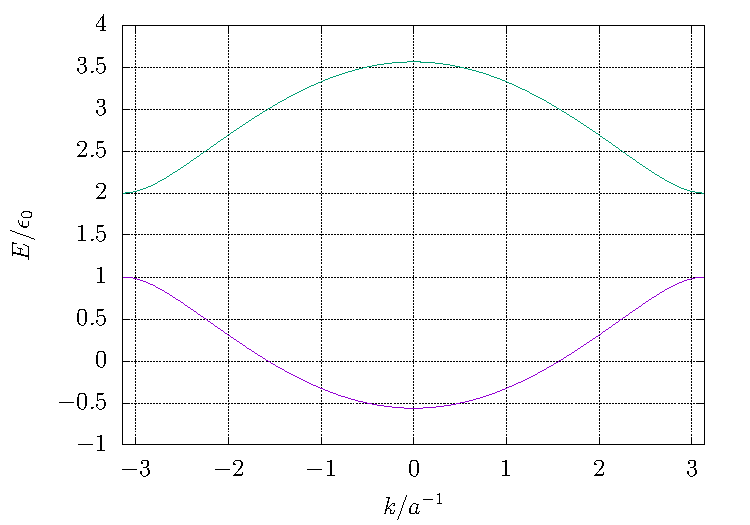
\includegraphics[width=.4\textwidth]{3-E-k-ReducedZoneScheme.pdf}}
            \subfigure[拓展布里渊区.]{
            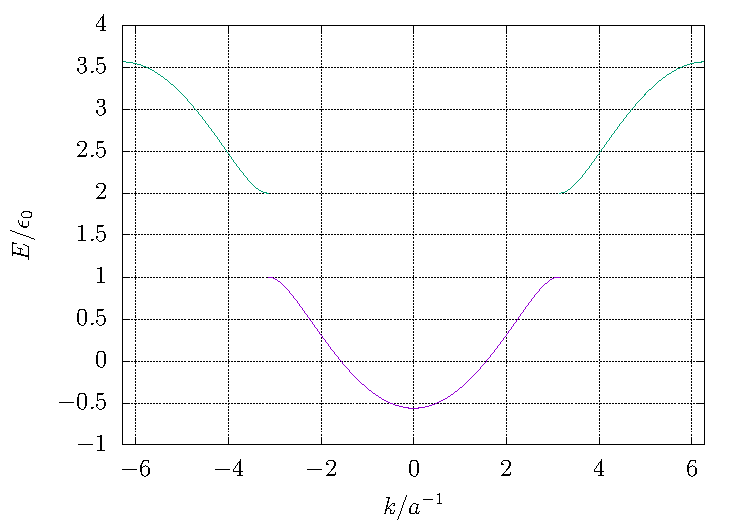
\includegraphics[width=.4\textwidth]{3-E-k-ExtendedZoneScheme.pdf}}
            \caption{色散关系的两种不同画法,其中$\epsilon_A=\epsilon_0$,$\epsilon_B=2\epsilon_0$,$t=0.5\epsilon_0$,横坐标$k$以$a^{-1}$为单位,纵坐标$\omega$以$\epsilon_0$为单位.}
            \label{3-E-k}
        \end{figure}
        \item[$\triangleright$] 当$\epsilon_A=\epsilon_B$时,系统由双原子链变为单原子链,色散关系可化为
        \begin{align}
            E=\epsilon_A\pm 2t\cos\left(\frac{ka}{2}\right).
        \end{align}
        两种模式的色散关系曲线在布里渊区边界处相连,如图\ref{3-E-k-2}.
        \begin{figure}[h]
            \centering
            \subfigure[简约布里渊区.]{
            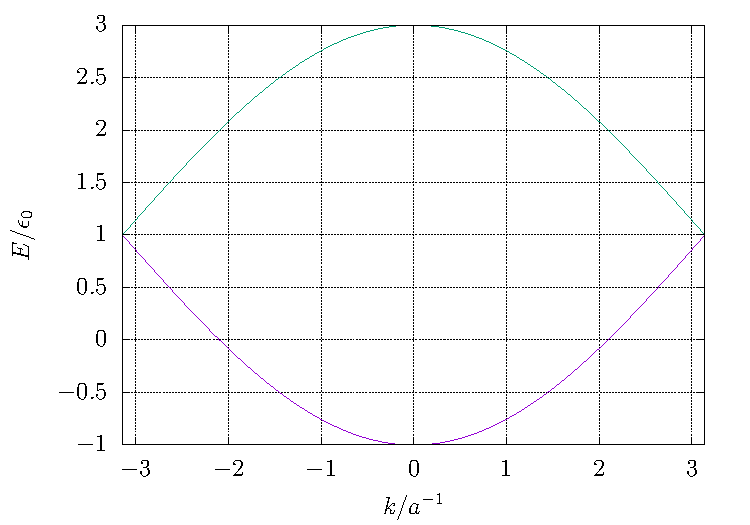
\includegraphics[width=.4\textwidth]{3-E-k-ReducedZoneScheme-2.pdf}}
            \subfigure[拓展布里渊区.]{
            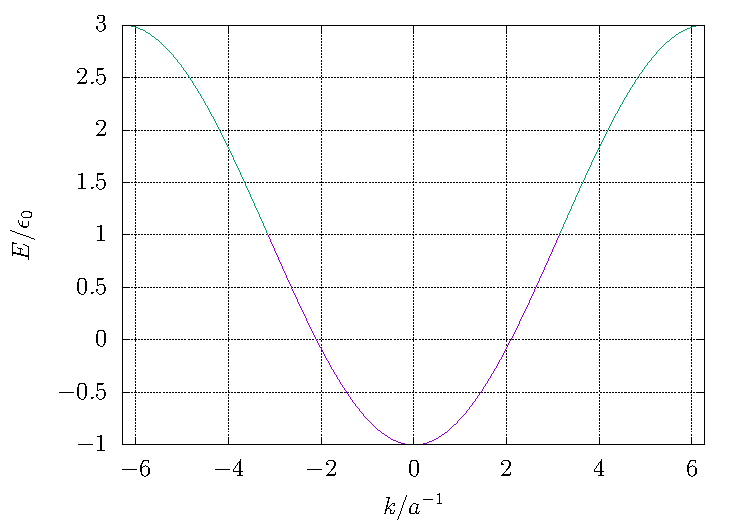
\includegraphics[width=.4\textwidth]{3-E-k-ExtendedZoneScheme-2.pdf}}
            \caption{色散关系的两种不同画法,其中$\epsilon_A=\epsilon_B=\epsilon_0$,$t=0.5\epsilon_0$,横坐标$k$以$a^{-1}$为单位,纵坐标$\omega$以$\epsilon_0$为单位.}
            \label{3-E-k-2}
        \end{figure}
        \item[$\triangleright$] 假设周期性边界条件中以$N$个原胞为周期,则共有$N$个$k$,每个$k$对应$2$个模式,也就是说一共有$2N$个能级,若每个原子仅有$1$个价电子,则共有$2N$个价电子,注意电子具有向上或向下的自旋,也就是说一个能级可填充$2$个自旋相反的电子,故低能带($N$个能级,$2N$个空位)被填充满,而高能带($N$个能级,$2N$个空位)为空. 系统的导电类型根据$\epsilon_A$和$\epsilon_B$之间的关系可大致分为以下三种情况:\\
        (1) 若沿用上一小题的条件,$\epsilon_A=\epsilon_B$,即没有带隙的话,则当施加电场,就可以产生电流,故该系统为\underline{导体}.\\
        (2) 若$\epsilon_A$和$\epsilon_B$有较小的差异,即带隙很小,则若需要产生电流,需要先消耗部分能量将电子激发到高能带上,此时系统为\underline{半导体}.\\
        (3) 若$\epsilon_A$和$\epsilon_B$之差很大,即带隙很大,则电子很难跃迁到高能带上而导电,此时系统为\underline{绝缘体}.
        \item[$\triangleright$] Li原子电负性极弱,而F原子电负性极强,也就是说对于LiF,$\epsilon_{Li}\gg\epsilon_{F}$,这导致两个模式的色散关系之间带隙极大,当施加电场时,处于低能带的电子很难跃迁至高能带,故很难产生电流,故LiF是极好的绝缘体.
    \end{itemize}
\end{sol}

\begin{prob}[(11.4) Two Orbital per Atom]
    \begin{enumerate}
        \item[(a)] Consider an atom with two orbitals, $A$ and $B$ having eigenenergies $\epsilon_{atomic}^A$ and $\epsilon_{atomic}^B$. Now suppose we make a one-dimensional chain of such atoms and let us assume that these orbitals remain orthogonal. We imagine hopping amplitudes $t_{AA}$ which allows an electron on orbital $A$ of a given atom to hop to orbital $A$ on the neighboring atom. Similarly we imagine a hopping amplitude $t_{BB}$ that allows an electron on orbital $B$ of a given atom to hop to orbital $B$ on the neighboring atom. (We assume that $V_0$, the energy shift of the atomic orbital due to neighboring atoms, is zero).
	\begin{itemize}
	    \item[$\triangleright$] Calculate and sketch the dispersion of the two resulting bands.
	    \item[$\triangleright$] If the atom is divalent, derive a condition on the quantities $\epsilon_{atomic}^A-\epsilon_{atomic}^B$, as well as $t_{AA}$ and $t_{BB}$ which determines whether the system is a metal or an insulator.
	\end{itemize}
	\item[(b)$^*$] Now suppose that there is in addition a hopping term $t_{AB}$ which allows an electron on one atom in orbital $A$ to hop to orbital $B$ on the neighboring atom  (and vice versa). What is the dispersion relation now?
    \end{enumerate}
\end{prob}
\begin{sol}
    \begin{enumerate}
        \item[(a)]
	\begin{itemize}
        \item[$\triangleright$] 电子的状态可表为
        \begin{align}
            \lvert\Psi\rangle=\sum_{n}\sum_{k\in\{A,B\}}\phi_{n,k}\lvert n,k\rangle,
        \end{align}
        其中$n$代表该状态下电子处于第$n$个原子上,$k=A$或$B$代表电子所处的原子轨道. 电子在一维固体中的总哈密顿为
        \begin{align}
            \hat{H}=\hat{H}_0+\hat{V}_h,
        \end{align}
        其中$\hat{H}_I$为电子处在某个独立原子中的哈密顿,根据题设,各个原子轨道正交归一,故有
        \begin{align}
            \langle m,j\rvert\hat{H}_0\lvert n,k\rangle=\epsilon_{atomic}^k\delta_{mn}\delta_{jk}.
        \end{align}
        $\hat{V}_h$为hopping energy,根据题设,相邻原子不同轨道之间不可hop,故
        \begin{align}
            \langle m,j\rvert\hat{V}_h\lvert n,k\rangle=t_{jj}(\delta_{m,n-1}+\delta_{m,n+1})\delta_{jk}.
        \end{align}
        故电子总哈密顿在$\{\lvert n,k\rangle\}$表象中的矩阵元为
        \begin{align}
            H_{(m,j)(n,k)}\langle m,j\rvert\hat{H}\lvert n,k\rangle=\langle m,j\rvert\hat{H}_0\lvert n,k\rangle+\langle m,j\rvert\hat{V}_h\lvert n,k\rangle=\epsilon_{atomic}^k\delta_{mn}\delta_{jk}-t_{jj}(\delta_{m,n-1}+\delta_{m,n+1})\delta_{jk}.
        \end{align}
        电子的薛定谔方程为
        \begin{align}
            \hat{H}\lvert\Psi\rangle=E\lvert\Psi\rangle.
        \end{align}
        因为相邻原子不同轨道之间不可hop,$A,B$两轨道完全不存在耦合. 在$\{\lvert n,k\rangle\}$表象中,薛定谔方程的线性代数形式本来应该有直积$\lvert n,k\rangle=\lvert n\rangle\otimes\lvert k\rangle$,现在我们可以分别对$k=A$和$k=B$列出方程
        \begin{align}
            \left(\begin{matrix}
                \epsilon_{atomic}^A & -t_{AA} &  &  & -t_{AA} \\
                -t_{AA} & \epsilon_{atomic}^A & -t_{AA} &  &  \\
                 &  \ddots & \ddots & \ddots &  \\
                 &  & -t_{AA} & \epsilon_{atomic}^A & -t_{AA} \\
                -t_{AA} &  &  & -t_{AA} & \epsilon_{atomic}^A
            \end{matrix}\right)\left(\begin{matrix}
                \phi_{1,A}\\
                \phi_{2,A}\\
                \vdots\\
                \phi_{N-1,A}\\
                \phi_{N,A}
            \end{matrix}\right)=&E_A\left(\begin{matrix}
                \phi_{1,A}\\
                \phi_{2,A}\\
                \vdots\\
                \phi_{N-1,A}\\
                \phi_{N,A}
            \end{matrix}\right),\\
            \left(\begin{matrix}
                \epsilon_{atomic}^B & -t_{BB} &  &  & -t_{BB} \\
                -t_{BB} & \epsilon_{atomic}^B & -t_{BB} &  &  \\
                 &  \ddots & \ddots & \ddots &  \\
                 &  & -t_{BB} & \epsilon_{atomic}^B & -t_{BB} \\
                -t_{BB} &  &  & -t_{BB} & \epsilon_{atomic}^B
            \end{matrix}\right)\left(\begin{matrix}
                \phi_{1,B}\\
                \phi_{2,B}\\
                \vdots\\
                \phi_{N-1,B}\\
                \phi_{N,B}
            \end{matrix}\right)=&E_B\left(\begin{matrix}
                \phi_{1,B}\\
                \phi_{2,B}\\
                \vdots\\
                \phi_{N-1,B}\\
                \phi_{N,B}
            \end{matrix}\right).
        \end{align}
        即
        \begin{align}
            -t_{AA}\phi_{n-1,A}+\epsilon_A\phi_{n,A}-t_{AA}\phi_{n+1,A}=&E_A\phi_{n,A},\\
            -t_{BB}\phi_{n-1,B}+\epsilon_B\phi_{n,B}-t_{BB}\phi_{n+1,B}=&E_B\phi_{n,B}.
        \end{align}
        设解为
        \begin{align}
            \phi_{n,A}=&Ae^{ikna},\\
            \phi_{n,B}=&Be^{ikna}.
        \end{align}
        其中$a$为原胞的长度. 将猜测的解代入薛定谔方程中得
        \begin{align}
            E_A=&\epsilon_A-t_{AA}(e^{-ika}+e^{ika})=\epsilon_A-2t_{AA}\cos ka,\\
            E_B=&\epsilon_B-t_{BB}(e^{-ika}+e^{ika})=\epsilon_B-2t_{BB}\cos ka.
        \end{align}
        色散关系如图\ref{4-E-k}.
        \begin{figure}[h]
            \centering
            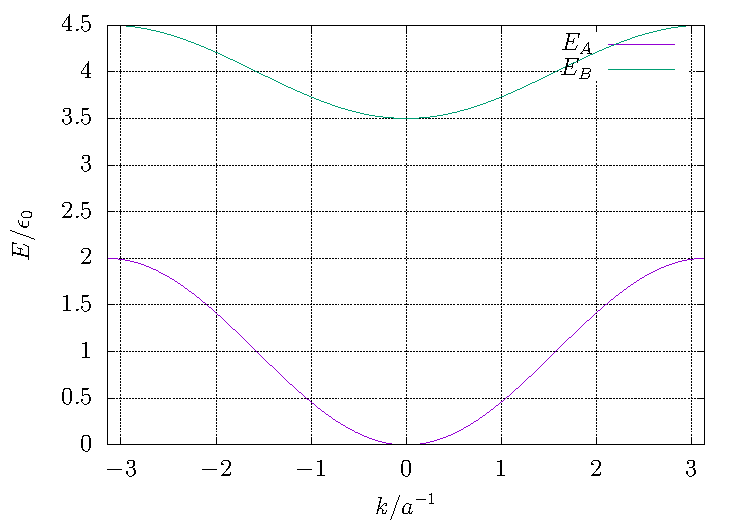
\includegraphics[width=.4\textwidth]{4-E-k.pdf}
            \caption{色散关系,其中$\epsilon_A=\epsilon_0$,$t_{AA}=0.5\epsilon_0$,$\epsilon_B=4\epsilon_0$,$t=0.25\epsilon_0$,横坐标$k$以$a^{-1}$为单位,纵坐标$\omega$以$\epsilon_0$为单位.}
            \label{4-E-k}
        \end{figure}
        \item[$\triangleright$] 设周期性边界条件中每个周期有$N$个原子,则共有$N$个$k$,每个$k$对应于电子在轨道$A$还是轨道$B$穿梭的两种模式,如果每个原子有$2$个价电子,则共有$2N$个价电子,注意电子具有向上或向下的自旋,也就是说一个能级可填充$2$个自旋相反的电子,故低能带($N$个能级,$2N$个空位)被填充满,而高能带($N$个能级,$2N$个空位)为空.\\
        (1) 若要使系统为导体,则应当没有带隙,也就是说两个能带有公共的能量范围:
        \begin{align}
            \epsilon_A+2\abs{t_{AA}}\geq\epsilon_B-2\abs{t_{BB}},
        \end{align}
        或
        \begin{align}
            \epsilon_B+2\abs{t_{BB}}\geq\epsilon_A-2\abs{t_{AA}},
        \end{align}
        即
        \begin{align}
            \abs{\epsilon_A-\epsilon_B}\leq 2(\abs{t_{AA}}+\abs{t_{BB}}).
        \end{align}
        (2) 若要使系统为导体,则两个能带没有公共的能量且应当有较大的带隙,即
        \begin{align}
            \abs{\epsilon_A-\epsilon_B}\gg 2(\abs{t_{AA}}+\abs{t_{BB}}).
        \end{align}
    \end{itemize}
    \item[(b)] 不同于上一小题,由于相邻原子不同轨道之间可hop,故有
    \begin{align}
        \langle m,j\rvert\hat{V}_h\lvert n,k\rangle=-t_{jj}(\delta_{m,n-1}+\delta_{m,n+1})\delta_{jk}-t_{kj}(1-\delta_{mn})(1-\delta_{jk}).
    \end{align}
    电子总哈密顿的矩阵元为
    \begin{align}
        \nonumber H_{(m,j)(n,k)}\langle m,j\rvert\hat{H}\lvert n,k\rangle=&\langle m,j\rvert\hat{H}_0\lvert n,k\rangle+\langle m,j\rvert\hat{V}_h\lvert n,k\rangle\\
        =&\epsilon_{atomic}^k\delta_{mn}\delta_{jk}-t_{jj}(\delta_{m,n-1}+\delta_{m,n+1})\delta_{jk}-t_{kj}(1-\delta_{mn})(1-\delta_{jk}).
    \end{align}
    线性代数形式的薛定谔方程为
    \begin{align}
        \left(\begin{matrix}
            \epsilon_{atomic}^A & 0 & -t_{AA} & -t_{BA} &  &  & -t_{AA} & -t_{BA} \\
            0 & \epsilon_{atomic}^B & -t_{AB} & -t_{BB} &  &  & -t_{AB} & -t_{BB} \\
            -t_{AA} & -t_{BA} & \epsilon_{atomic}^A & 0 & -t_{AA} & -t_{BA} &  &  \\
            -t_{AB} & -t_{BB} & 0 & \epsilon_{atomic}^B & -t_{AB} & -t_{BB} &  &  \\
            &  & \ddots & \ddots & \ddots & \ddots & \ddots & \ddots \\
            &  & \ddots & \ddots & \ddots & \ddots & \ddots & \ddots \\
            -t_{AA} & -t_{BA} &  &  & -t_{AA} & -t_{BA} & \epsilon_{atomic}^A & 0 \\
            -t_{AB} & -t_{BB} &  &  & -t_{AB} & -t_{BB} & 0 & \epsilon_{atomic}^B
        \end{matrix}\right)\left(\begin{matrix}
            \phi_{1,A}\\
            \phi_{1,B}\\
            \phi_{2,A}\\
            \phi_{2,B}\\
            \vdots\\
            \vdots\\
            \phi_{N,A}\\
            \phi_{N,B}
        \end{matrix}\right)=&E\left(\begin{matrix}
            \phi_{1,A}\\
            \phi_{1,B}\\
            \phi_{2,A}\\
            \phi_{2,B}\\
            \vdots\\
            \vdots\\
            \phi_{N,A}\\
            \phi_{N,B}
        \end{matrix}\right),
    \end{align}
    即
    \begin{align}
        -t_{AA}\phi_{n-1,A}-t_{BA}\phi_{n-1,B}+\epsilon_{atomic}^A\phi_{n,A}-t_{AA}\phi_{n+1,A}-t_{BA}\phi_{n+1,B}=&E\phi_{n,A},\\
        -t_{AB}\phi_{n-1,A}-t_{BB}\phi_{n-1,B}-\epsilon_{atomic}^B\phi_{n,B}-t_{AB}\phi_{n+1,A}-t_{AB}\phi_{n+1,B}=&E\phi_{n,B}.
    \end{align}
    设解为
    \begin{align}
        \phi_{n,A}=&Ae^{ikna},\\
        \phi_{n,B}=&Be^{ikna}.
    \end{align}
    将猜测的解代入薛定谔方程中得
    \begin{align}
        [\epsilon_{atomic}^A-t_{AA}(e^{-ika}+e^{ika})]A-t_{BA}B(e^{-ika}+e^{ika})=EA,\\
        [\epsilon_{atomic}^B-t_{BB}(e^{-ika}+e^{ika})]B-t_{AB}A(e^{-ika}+e^{ika})=EB.
    \end{align}
    即
    \begin{align}
        \left(\begin{matrix}
            \epsilon_{atomic}^A-2t_{AA}\cos ka&-2t_{BA}\cos ka\\
            -2t_{AB}\cos ka&\epsilon_{atomic}^B-2t_{BB}\cos ka
        \end{matrix}\right)\left(\begin{matrix}
            A\\
            B
        \end{matrix}\right)=E\left(\begin{matrix}
            A\\
            B
        \end{matrix}\right).
    \end{align}
    下面求解上式左边这个矩阵的本征值
    \begin{align}
        \nonumber&\abs{\begin{matrix}
            \epsilon_{atomic}^A-2t_{AA}\cos ka-E&-2t_{BA}\cos ka\\
            -2t_{AB}\cos ka&\epsilon_{atomic}^B-2t_{BB}\cos ka-E
        \end{matrix}}=E^2-[\epsilon_{atomic}^A+\epsilon_{atomic}^B-2(t_{AA}+t_{BB})\cos ka]E\\
        &+[\epsilon_{atomic}^A\epsilon_{atomic}^B-2(\epsilon_{atomic}^At_{BB}+\epsilon_{atomic}^Bt_{AA})\cos ka+4(t_{AA}t_{BB}-t_{BA}t_{AB})\cos^2ka]=0
    \end{align}
    解得色散关系为
    \footnotesize
    \begin{align}
        \nonumber&E_{pm}=\frac{1}{2}\{[\epsilon_{atomic}^A+\epsilon_{atomic}^B-2(t_{AA}+t_{BB})\cos ka]\\
        &\pm\sqrt{[\epsilon_{atomic}^A+\epsilon_{atomic}^B-2(t_{AA}+t_{BB})\cos ka]^2-4[\epsilon_{atomic}^A\epsilon_{atomic}^B-2(\epsilon_{atomic}^At_{BB}+\epsilon_{atomic}^Bt_{AA})\cos ka+4(t_{AA}t_{BB}-t_{BA}t_{AB})\cos^2ka]}.
    \end{align}
    \normalsize
    \end{enumerate}
\end{sol}

\begin{prob}[(11.8) Peierls Distortion$^*$]
    Consider a chain made up of all the same type of atom, but in such a way that the spacing between atoms alternates as long-short-long-short as follows
    \[
        -A=A-A=A-A=A-
    \]
    In a tight binding model, the shorter bonds (marked with $=$) will have hopping matrix element $t_{short}=t(1+\epsilon)$ whereas the longer bonds (marked with $-$) have hopping matrix element $t_{long}=t(1-\epsilon)$. Calculate the tight-binding energy spectrum of this chain. (The onsite energy $\epsilon$ is the same on every atom). Expand your result to linear order in $\epsilon$. Suppose the lower band is filled and the upper band is empty (what is the valence of each atom in this case?). Calculate the total ground-state energy of the filled lower band, and show it decreases linearly with increasing $\epsilon$.\\
    Now consider a chain of equally spaced identical $A$ atoms connected together with identical springs with spring constant $\kappa$. Show that making a distortion whereby alternating spring are shorter / longer by $\delta x$ costs energy proportional to $(\delta x)^2$. Conclude that for a chain with the valence as in the first part of the problem, a distortion of this sort will occur spontaneously. This is known as a Peierls distortion.
\end{prob}
\begin{sol}
    下面称左边为长键、右边为短键的原子为I类原子,左边为短键、右边为长键的原子为II类原子. 该原子链中一个I类原子和一个II类原子组成一个原胞($-A=A$). 设原子处于第$n$个原胞中的$k$类原子上的状态为$\lvert n,k\rangle$. 电子的状态可表为
    \begin{align}
        \lvert\Psi\rangle=\sum_n\sum_{k\in\{I,II\}}\phi_{n,k}\lvert n,k\rangle.
    \end{align}
    电子在一维固体中的总哈密顿为
    \begin{align}
        \hat{H}=\hat{H}_0+\hat{V}_h,
    \end{align}
    其中$\hat{H}_0$为电子处在某个独立原子中的哈密顿:
    \begin{align}
        \langle m,j\rangle\hat{H}_0\lvert n,k\rangle=\epsilon_0,
    \end{align}
    (题设中为$\epsilon$,但是$\epsilon$和描述不同键hopping energy差异的无量纲常数混了,故此处重新定义)\\
    而$\hat{V}_h$为hopping energy:
    \begin{align}
        \langle m,j\rvert\hat{V}_h\lvert n,k\rangle=\left\{\begin{array}{ll}
            -t(1-\epsilon),&m=n-1,k=I,j=II,\\
            -t(1-\epsilon),&m=n,k=I,j=II,\\
            -t(1+\epsilon),&m=n,k=II,j=I,\\
            -t(1+\epsilon),&m=n+1,k=II,j=I,\\
            0,&\text{otherwise}.
        \end{array}\right.
    \end{align}
    电子的薛定谔方程为
    \begin{align}
        \hat{H}\lvert\Psi\rangle=E\lvert\Psi\rangle.
    \end{align}
    在$\{\lvert n,k\rangle\}$表象中,薛定谔方程的线性代数形式为
    \begin{align}
        \left(\begin{matrix}
            \epsilon_0 & -t(1+\epsilon) &  &  &  &  & -t(1-\epsilon) \\
                -t(1+\epsilon) & \epsilon_0 & -t(1-\epsilon) &  &  &  &  \\
                 & -t(1-\epsilon) & \epsilon_0 & -t(1+\epsilon) &  &  &  \\
                 &  & -t(1+\epsilon) & \epsilon_0 & -t(1-\epsilon) &  &  \\
                 &  &  & \ddots & \ddots & \ddots &  \\
                 &  &  &  & -t(1-\epsilon) & \epsilon_0 & -t(1+\epsilon) \\
                 -t(1-\epsilon) &  &  &  &  & -t(1+\epsilon) & \epsilon_0
        \end{matrix}\right)\left(\begin{matrix}
            \phi_{1,I}\\
            \phi_{1,II}\\
            \phi_{2,I}\\
            \phi_{2,II}\\
            \ddots\\
            \phi_{N,I}\\
            \phi_{N,II}
        \end{matrix}\right)=&E\left(\begin{matrix}
            \phi_{1,I}\\
            \phi_{1,II}\\
            \phi_{2,I}\\
            \phi_{2,II}\\
            \ddots\\
            \phi_{N,I}\\
            \phi_{N,II}
        \end{matrix}\right),
    \end{align}
    即
    \begin{align}
        -t(1-\epsilon)\phi_{n-1,II}+\epsilon_0\phi_{n,I}-t(1+\epsilon)\phi_{n,II}=&E\phi_{n,I},\\
        -t(1+\epsilon)\phi_{n,I}+\epsilon_0\phi_{n,II}-t(1-\epsilon)\phi_{n+1,I}=&E\phi_{n,II}.
    \end{align}
    设解为
    \begin{align}
        \phi_{n,I}=A_Ie^{ika},\\
        \phi_{n,II}=A_{II}e^{ika}.
    \end{align}
    其中$a$为原胞的长度. 将猜测的解代入薛定谔方程中得
    \begin{align}
        \epsilon_0A_I-t[(1+\epsilon)+(1-\epsilon)e^{-ika}]A_{II}=EA_I,\\
        \epsilon_0A_{II}-t[(1+\epsilon)+(1-\epsilon)e^{ika}]A_{II}=EA_{II},
    \end{align}
    即
    \begin{align}
        \left(\begin{matrix}
            \epsilon_0&-t[(1+\epsilon)+(1-\epsilon)e^{-ika}]\\
            -t[(1+\epsilon)+(1-\epsilon)e^{ika}]&\epsilon_0
        \end{matrix}\right)\left(\begin{matrix}
            A_I\\
            A_{II}
        \end{matrix}\right)=E\left(\begin{matrix}
            A_I\\
            A_{II}
        \end{matrix}\right).
    \end{align}
    下面求解上式左边这个矩阵的本征值
    \begin{align}
        \abs{\begin{matrix}
            \epsilon_0-E&-t[(1+\epsilon)+(1-\epsilon)e^{-ika}]\\
            -t[(1+\epsilon)+(1-\epsilon)e^{ika}]&\epsilon_0-E
        \end{matrix}}=E^2-2\epsilon_0E+\epsilon_0^2-2t^2[1+\epsilon^2+(1-\epsilon^2)\cos ka]=0.
    \end{align}
    解得色散关系为
    \begin{align}
        \nonumber E_{\pm}(k)=&\epsilon_0\pm t\sqrt{2[1+\epsilon^2+(1-\epsilon^2)\cos ka]}\\
        =&\epsilon_0\pm 2t\sqrt{\epsilon^2+(1-\epsilon^2)\cos^2\left(\frac{ka}{2}\right)}
    \end{align}
    题目要求将色散关系展开到关于$\epsilon$一阶项,但是我们发现一阶项的系数为$0$,故我们只好将色散关系关于$\epsilon$展开到二阶项得
    \begin{align}
        \nonumber E_{\pm}\approx\epsilon_0\pm 2t\left[\cos\left(\frac{ka}{2}\right)+\frac{\sin^2\left(\frac{ka}{2}\right)}{\abs{\cos\left(\frac{ka}{2}\right)}}\epsilon^2\right]
    \end{align}
    设周期性边界条件中以$N$个原胞为周期. 当每个原子有$1$个价电子时,低能带被填满而高能带为空,总的基态能量为
    \begin{align}
        \nonumber E_g=&2\int_{-\pi/a}^{\pi/a}\frac{Na\,dk}{2\pi}E_-(k)\\
        \nonumber=&\frac{Na}{\pi}\int_0^{2\pi/a}dk\,\left\{\epsilon_0-2t\left[\cos\left(\frac{ka}{2}\right)+\frac{\sin^2\left(\frac{ka}{2}\right)}{\abs{\cos\left(\frac{ka}{2}\right)}}\epsilon^2\right]\right\}\\
        \nonumber=&N\epsilon_0-\epsilon^2\frac{2Nat}{\pi}\int_{-\pi/a}^{\pi/a}dk\,\frac{\sin^2\left(\frac{ka}{2}\right)}{\abs{\cos\left(\frac{ka}{2}\right)}}.
    \end{align}
    其中$\frac{\sin^2\left(\frac{ka}{2}\right)}{\abs{\cos\left(\frac{ka}{2}\right)}}$实际上是发散到无穷大,当然这在物理上不可能,但这告诉我们它至少将是一个很大常数,因此系统的基态能量随着$\epsilon$增加而降低(很多).\\
    对于一个由相同原子、相同劲度系数的弹簧组成原子链,当其中的某一个片段从$-A-A-A-$变为$-A=A--A-$(中间原子向左移动$\delta x$)时增加能量
    \begin{align}
        \Delta E=\kappa(\delta x)^2.
    \end{align}
    它仅为$(\delta x)^2$或者说($\epsilon^2$)的有限倍. 因此,由于这种畸变使得系统基态能量降低应当大于随之产生的势能上升,因此会自发产生.\\
    (可能最后部分数学上处理得很不严谨,但是物理图像大致应当不错,请见谅.)
\end{sol}
\end{document}